\documentclass[11pt,a4paper]{article}
\usepackage[czech]{babel}
\usepackage[utf8]{inputenc}
\usepackage[left=2cm,text={17cm, 24cm},top=3cm]{geometry}
\usepackage{multirow}
\usepackage[longend,linesnumbered,ruled]{algorithm2e}
\usepackage{graphics}
\usepackage{picture}
\usepackage{pdflscape}
\usepackage{times}
\usepackage{ragged2e}
\usepackage[skip=0pt]{caption}
\newcommand{\myuv}[1]{\quotedblbase #1\textquotedblleft}

\begin{document}

\begin{titlepage}
\begin{center}
\Huge
\textsc{
    Vysoké učení technické v~Brně \\ [-.25em]
    \huge Fakulta informačních technologií}\\
\vspace{\stretch{0.382}}
\LARGE
Typografie a publikování -- 3. projekt \\ [-.25em]
\Huge Tabulky a obrázky \\
\vspace{\stretch{0.618}}

{\Large \today \hfill
Jakub Kulich}
\end{center}
\end{titlepage}

\section{Úvodní strana}
Název práce umístěte do zlatého řezu a nezapomeňte uvést dnešní datum a vaše jméno a príjmení.

\section{Tabulky}
Pro sázení tabulek můžeme použít buď prostředí \texttt{tabbing} nebo prostředí \texttt{tabular}.
\subsection{Prostředí \texttt{tabbing}}
Při použití \texttt{tabbing} vypadá tabulka následovně:
\begin{tabbing}
    Vodní melouny \quad \= xx,xx  \quad \= 1~kus \kill
    \textbf{Ovoce} \> \textbf{Cena} \> \textbf{Množství} \\
    Jablka \> 25,90 \> 3~kg \\
    Hrušky \> 27,40 \> 2,5~kg \\
    Vodní melouny \> 35 \> 1~kus \\
\end{tabbing}

\noindent
Toto prostředí se dá také použít pro sázení algoritmů, ovšem vhodnější je použít 
prostředí \texttt{algorithm} nebo \texttt{algorithm2e} (viz sekce \ref{sec:algo}).

\subsection{Prostředí \texttt{tabular}}
Další možností, jak vytvořit tabulku, je použít prostředí \texttt{tabular}. Tabulky pak 
budou vypadat takto\footnote{Kdyby byl problem s~\texttt{cline}, zkuste se podívat třeba sem: 
http://www.abclinuxu.cz/tex/poradna/show/325037.}:
\begin{table}[h]
    \catcode`\-=12
    \begin{center}
    \begin{tabular}{|l|r|r|}
        \hline
        & \multicolumn{2}{|c|}{\bf Cena} \\ \cline{2-3}
        \bf Měna & \bf nákup & \bf prodej \\ \hline
        EUR & 27,34 & 27,42 \\
        GBP & 33,09 & 33,21 \\
        USD & 19,87 & 19,95 \\ \hline
    \end{tabular}
    \end{center}
    \caption{Tabulka kurzů k~dnešnímu dni}
    \label{tab1}
\end{table}
\begin{table}[h]
    \catcode`\-=12
    \begin{center}
    \begin{tabular}{|c|c|}
        \hline
        A~& $\neg$ A~\\ \hline
        P & N \\ \hline
        O~& O~\\ \hline
        X & X \\ \hline
        N & P \\ \hline
    \end{tabular}
    \begin{tabular}{|c|c|c|c|c|c|}
        \hline
        \multicolumn{2}{|c|}{\multirow{2}{*}{A $\wedge$ B}} & \multicolumn{4}{|c|}{B} \\ \cline{3-6}
        \multicolumn{2}{|c|}{} & \bf P & \bf O~& \bf X & \bf N \\ \hline
        \multirow{4}{*}{A} & \bf P &  P &  O~&  X &  N \\ \cline{2-6}
        \multirow{4}{*}{} & \bf O~&  O~&  O~&  N &  N \\  \cline{2-6}
        \multirow{4}{*}{} & \bf X &  X &  N &  X &  N \\  \cline{2-6}
        \multirow{4}{*}{} & \bf N &  N &  N &  N &  N \\  \cline{2-6}
        \hline
    \end{tabular}
    \begin{tabular}{|c|c|c|c|c|c|}
        \hline
        \multicolumn{2}{|c|}{\multirow{2}{*}{A $\vee$ B}} & \multicolumn{4}{|c|}{B} \\ \cline{3-6}
        \multicolumn{2}{|c|}{} & \bf P & \bf O~& \bf X & \bf N \\ \hline
        \multirow{4}{*}{A} & \bf P &  P &  P &  P &  P \\ \cline{2-6}
        \multirow{4}{*}{} & \bf O~&  P &  O~&  P &  O~\\  \cline{2-6}
        \multirow{4}{*}{} & \bf X &  P &  P &  X &  X \\  \cline{2-6}
        \multirow{4}{*}{} & \bf N &  P &  O~&  X &  N \\  \cline{2-6}
        \hline
    \end{tabular}
    \begin{tabular}{|c|c|c|c|c|c|}
        \hline
        \multicolumn{2}{|c|}{\multirow{2}{*}{A $\to$ B}} & \multicolumn{4}{|c|}{B} \\ \cline{3-6}
        \multicolumn{2}{|c|}{} & \bf P & \bf O~& \bf X & \bf N \\ \hline
        \multirow{4}{*}{A} & \bf P &  P &  O~&  X &  N \\ \cline{2-6}
        \multirow{4}{*}{} & \bf O~&  P &  O~&  P &  O~\\  \cline{2-6}
        \multirow{4}{*}{} & \bf X &  P &  P &  X &  X \\  \cline{2-6}
        \multirow{4}{*}{} & \bf N &  P &  P &  P &  P \\  \cline{2-6}
        \hline
    \end{tabular}
    \end{center}
    \caption{Protože Kleeneho trojhodnotová logika už je \myuv{zastaralá}, uvádíme si zde příklad čtyřhodnotové logiky}
    \label{tab2}
\end{table}

\clearpage
\section{Algoritmy} \label{sec:algo}
Pokud budeme chtít vysázet algoritmus, můžeme použít prostředí \texttt{algorithm}\footnote{\raggedright Pro nápovědu, jak zacházet s~prostředím algorithm, můžeme zkusit tuhle stránku: http://ftp.cstug.cz/pub/tex/CTAN/macros/latex/contrib/algorithms/algorithms.pdf.} nebo \texttt{algorithm2e}\footnote{Pro algorithm2e zase tuhle: http://ftp.cstug.cz/pub/tex/CTAN/macros/latex/contrib/algorithm2e/algorithm2e.pdf.
}.

\noindent
Příklad použití prostředí \texttt{algorithm2e} viz Algoritmus \ref{alg1}

\IncMargin{1em}
\begin{algorithm}[h]
    \SetAlgorithmName{Algoritmus}{algo}{algolist}
    \SetAlgoNoLine
    \caption{\textsc{FastSLAM}}
    \label{alg1}
    \Indm
    \KwIn{$(X_{t-1}, u_t, z_t)$}
    \KwOut{$X_t$}
    \Indp
    \SetNlSty{textrm}{}{:}
    $\overline{X_t} = X_t = 0$

    \For{$k = 1$ to $M$}{
        $x_t^{[k]} = \textit{sample\_motion\_model}(u_t,x_{t-1}^{[k]})$

        $\omega_t^{[k]} = \textit{measurement\_model}(z_t,x_{t}^{[k]},m_{t-1})$

        $m_t^{[k]} = updated\_occupacny\_grid(z_t,x_{t}^{[k]},m_{t-1}^{[k]})$

        $\overline{X_t} = \overline{X_t} + \langle x_x^{[m]},\omega_t^{[m]}\rangle $

    }
    \For{$k = 1$ to $M$}{
        draw $i$ with probability $\approx \omega_t^{[t]}$

        add $\langle x_x^{[k]},m_t^{[k]}\rangle $ to $X_t$
    }
    \KwRet{$X_t$}
                                                                        
\end{algorithm}



\section{Obrázky}
Do našich článků můžeme samozřejmě vkládat obrázky. Pokud je obrázkem fotografie,
můžeme klidně použít bitmapový soubor. Pokud by to ale mělo být nějaké schéma nebo
něco podobného, je dobrým zvykem takovýto obrázek vytvořit vektorově.
\begin{figure}[h]
    \begin{center}
        \scalebox{0.4}{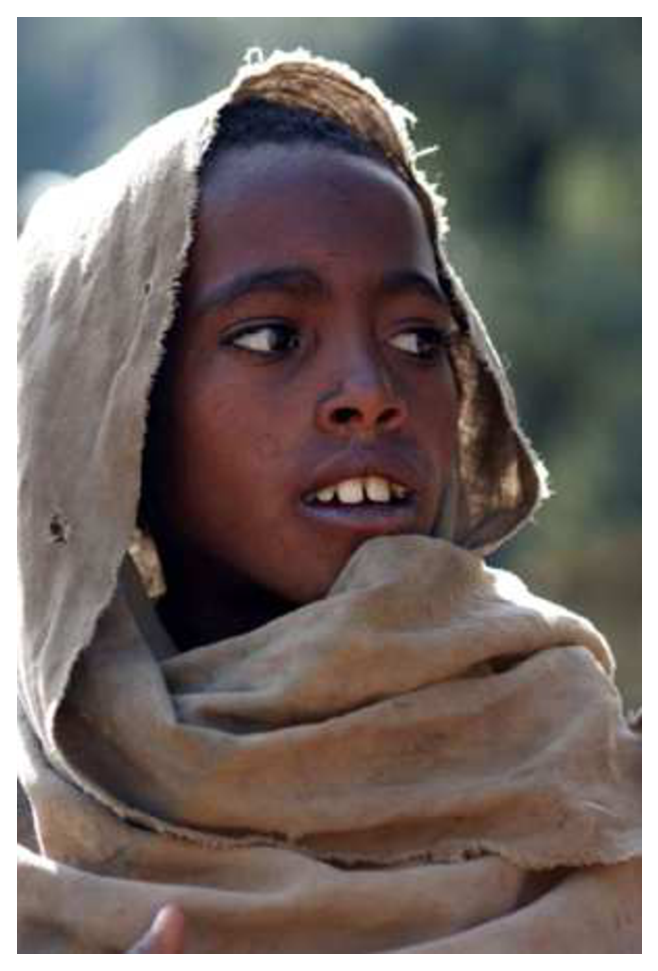
\includegraphics{etiopan}} 
        \reflectbox{\scalebox{0.4}{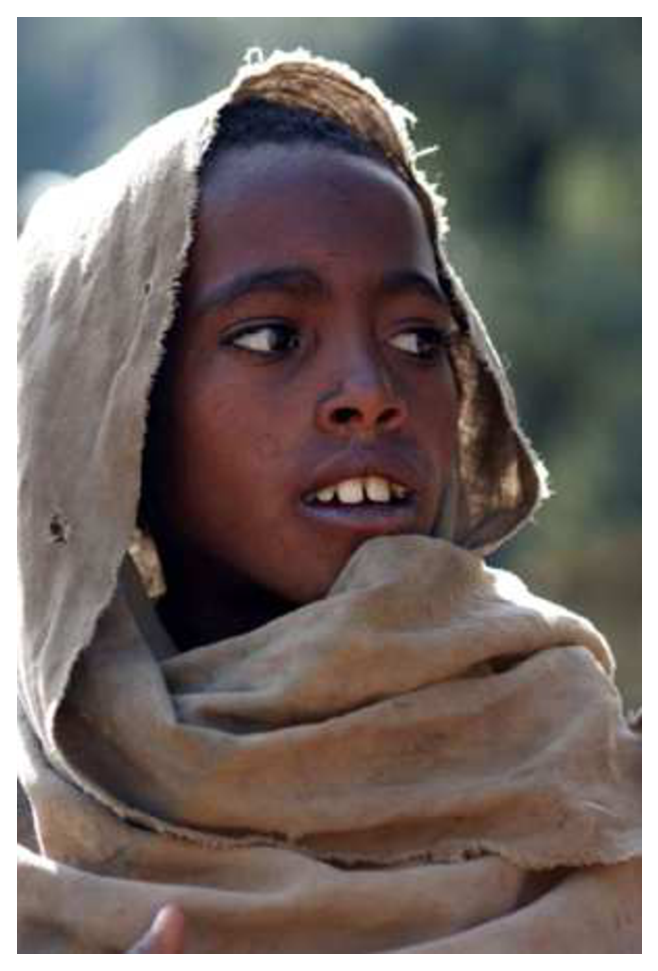
\includegraphics{etiopan}}}
    \end{center}
    \caption{Malý Etiopánek a jeho bratříček}
    \label{obr1}
\end{figure}

\clearpage
Rozdíl medzi vektorovým \ldots
\begin{figure}[h]
    \begin{center}
        \scalebox{0.4}{
\includegraphics{oniisan}}
    \end{center}
    \caption{Vektorový obrázek}
    \label{obr2}
\end{figure}

\noindent
\ldots a bitmapovým obrázkem.
\begin{figure}[h]
    \begin{center}
        \scalebox{.6}{
\includegraphics{oniisan2}}
    \end{center}
    \caption{Bitmapový obrázek}
    \label{obr3}
\end{figure}


\noindent
se projeví například  při zvětšení.


Odkazy (nejen ty) na obrázky \ref{obr1}, \ref{obr2} a \ref{obr3}, na  
tabulky \ref{tab1} a \ref{tab2} a také na algoritmus \ref{alg1} jsou udělány pomocí 
křížových odkazů. Pak je ovšem potřeba zdrojový soubor přeložit dvakrát.


Vektorové obrázky lze vytvořit i přímo v~LATEXu, například pomocí prostředí 
\texttt{picture}. 

\begin{landscape}
    \begin{figure}
    \begin{picture}(200mm,6cm)(-40,-10)
        \linethickness{4pt}
        \put(0.5cm,1.4cm){\line(1,0){19cm}}

        \linethickness{1.1pt}
        \put(2.5cm,1.4cm){\line(0,1){3.6cm}}
        \put(2.5cm,5cm){\line(1,0){4.2cm}}
        \put(6.7cm,4.5cm){\line(0,1){1cm}}
        \put(12.7cm,4.5cm){\line(0,1){1cm}}
        \put(6.7cm,5.5cm){\line(1,0){6cm}}
        \put(4.5cm,4.5cm){\line(1,0){14cm}}
        \put(12.7cm,4.7cm){\line(1,0){4.8cm}}
        \put(17.5cm,4.5cm){\line(0,1){0.2cm}}
        \put(4.5cm,3.9cm){\line(1,0){14cm}}
        \put(4.5cm,3.9cm){\line(0,1){0.6cm}}
        \put(18.5cm,3.9cm){\line(0,1){0.6cm}}
        \put(3.5cm,1.4cm){\line(0,1){1.4cm}}
        \put(3.5cm,2.8cm){\line(1,0){3.5cm}}
        \put(7.3cm,2.7cm){\line(0,1){1cm}}
        \put(7.3cm,3.7cm){\line(1,0){11cm}}
        \put(8.5cm,2.3cm){\line(1,0){10cm}}
        \put(18.3cm,2.3cm){\line(0,1){1.4cm}}
        \put(18.5cm,1.4cm){\line(0,1){0.9cm}}
        \put(17.3cm,8cm){\circle{40}}
        \thicklines
        \put(4.5cm,3.9cm){\line(1,-1){1.1cm}}
        \put(7cm,2.8cm){\line(3,-1){4cm}}
        \framebox(200mm,10cm){}

    \end{picture}
        \caption{Vektorový obrázek v~prostředí \texttt{picture}}
    \end{figure}
\end{landscape}
\end{document}
